% !TEX root = ./Thesis.tex

\chapter{Micro-NMR}

All NMR experiments depend on two performance metrics: sensitivity and resolution. Sensitivity
here means the minimum number of spins needed to give a signal clearly above the noise. Resolution
quantifies how well different spins in the sample can be differentiated. These two properties
are often linked, by selecting a smaller sample it is possible to enhance resolution by detecting
a smaller portion of spins in the sample but this compromises sensitivity as the number of spins become more
limited.

 In NMR, the long life time of the nuclear spin states (minutes in some cases) contirbute to extremely
 narrow lines in the spectrum with resolutions of one part per billion regularly acheived in
 commercial systems.

 \section{Sensitivity}

 \subsection{Signal to noise ratio}


 Sensitivity in NMR at thermal equilibrium is always in short supply. In an NMR experiment the signal
 is proportional to the net magnetisation, $M_0$, of the sample\citep{webb2005nmr}:
\begin{equation}\label{eqn:Webb}
  M_0 = \frac{\gamma~h}{4\pi}(I(I+1))(P_{\alpha}-P_{\beta}) = N\gamma^2\hbar^2I(I+1)\frac{B_0}{3k_BT}
\end{equation}
where $\gamma$ is the gyromagnetic ratio of the nucleus,$\hbar$ is Plankc's constant $h$/2\pi, $P_{\alpha}-P_{\beta}$ is the population difference between zeeman energy levels seen in \ref{Population}, $B_0$ is the magnetic field, $N$ is
the number of spins per unit volume , $k_B$ is the Boltzmann constant and T is the absolute temperature. The magnetisation
and therefore signal depends on the population difference which at room temperature is on the order of $10^{-25}$J
which is much lower that the thermal energy of the system. From the equation, increasing $B_0$ would seem a
valid strategy and comparatively it can be, increasing from 14.1T to 23.5T can almost double the signal,
however even at 23.5T there is only a factor of ~$6\times10-6$ in population difference. It's this
very small value that is responsible for the low sensitivity of NMR compared to other techniques.

Detection in NMR is typically done through the induction of a voltage in a coil that's close
to the precessing nuclear spins this is usually referred to as the sample coil. Unfortunately,
this coil also brings with it a type of interference, noise, analagous to the 'hiss' in the backgound
of radio it is produced mainly from thermal motion of electrons in the sample coil with some contribution from thermal
motion of ions in solution. The signal to noise ratio, SNR, is an important factor in NMR experiments if its too low
the signal will never be seen.

The SNR was formulated by Abragam\citep{Abragam:1961vg} and the analysis extended by Hoult and
Richards\citep{Hoult:1976dw} and is defined as the peak signal divided by the root mean square (rms) noise including the magnetisation from \ref{eqn:Webb} we find\citep{vanBentum:2007fda}:
\begin{equation}
  \text{SNR} = \frac{k_0\frac{B_1}{i}V_s\omega_0\frac{1}{\sqrt{2}}M}{F\sqrt{4k_BTR_{\text{noise}}\Delta~f}}
\end{equation}
where $k_0$ is a contant that accounts for spatial inhomogeneities in the $B_1$ field, $V_s$ is the sample volume,
$\omega_0$ is the larmour frequency, the factor $\frac{1}{\sqrt{2}}$ is introduced as the noise is rms noise. The
factor $B_1/i$ the magnetic field from the coil per unit current is defined as the coil sensitivity. The denominator is
the noise determined by the noise factor from the spectrometer ($F$) and the dissipative loses ($R_{\text{noise}}$) of
the coil, circuit and sample for the spectral bandwidth $\Delta~f$. T is the absolute temperature and $k_b$ is the
boltzmann constant.

In the same paper, Hoult and Richards introduced the principle of reciprocity for calculating the
sensitivity of the RF coil, This states that the signal received from a sample by a coil is proportional to the magnetic
field which would have been created in the sample if unit current were passed through the coil. Therefore the SNR is
directly proportional to the sensitivity of the coil, $B_1/i$. This can be seen if we define an
effective sample volume $V'_s = k_0V_s$ that is the volume in which $B_1$ is within 10\% of the maximum
value at the center of the coil. The SNR is given by a more simple expression\citep{vanBentum:2007fda}:
\begin{equation}
  SNR = C\frac{B_1N_s}{i\sqrt{R\Delta~f}}
\end{equation}
where $N_s$ is the number of spins in located within an effective volume $V'_s$.
For protons at 600MHz the constant, $C$ equals $1.4\times10^{-11}$ in SI units ($B_0$ = 14.1T, $T$ = 300K, $\gamma$ =
$0.2675\times10^9$ $\text{rad} \text{T}^{-1}\text{s}^{-1}$, $I = 1/2$ and $F = 1$ assuming neglible noise from the spectrometer.)

From the simple expression it becomes clear that the way to improve SNR is to increase the filling factor
(optimize the number of spins in the number of spins in $B_1$), maximise coil sensitivity, $B_1/i$, and
minimise the total resistance. The filling factor, $\alpha_F$ is given by:
\begin{equation}\label{eqn:FillingFactor}
  \alpha_F = \frac{\int~B_1^2\rho(r)dV}{\int~B_1^2dV}
\end{equation}
where the function $\rho$ is unity in the sample area, and zero elsewhere. For a long solenoid coil with the
interior space filled with sample, $\alpha_F = 1/2$. Most other desings have a lower filling factor.

Two of these three can be solved by decreasing the size of the detector. The third, minimising resistance
can be tackled by commercially available cryoprobes where the coil is cooled with a stream of He gas to
~20K this reduces the thermal noise from the source and can increase SNR by a factor of four.

To see how size of coil affects SNR we take an RF helical coil. An idealised coil
is a cylindrical shell with uniform current density. The RF current penetrates to a frequency
specific depth $\delta$. For copper at 600 MHz and room temperature $\delta$ = 2.7 $\mu$m. The center
field is given by:
\begin{equation}
  \frac{B_1}{i} = \frac{\mu_0}{\sqrt{l^2+d^2}}
\end{equation}
Resistance is:
\begin{equation}
  R = \rho\frac{\pi~d}{l\delta}
\end{equation}
with l, the height of the copper cylinder, d the diameter and $\rho$ the resistivity.
Optimum coil sensitivity is given by $d/l$ = $1$ in this case the signal to noise is:
\begin{equation}
  SNR = 0.9\times10^-16\frac{N_s}{d\sqrt{\delta~f}}
\end{equation}
For a fixed number of spins the SNR scales with 1/d as predicted by \citep{Hoult:1976dw}

\section{Limit of Detection}

The signal to noise ratio can be found in the time or frequency domain. In the time domain the noise, $N$, is
~$\sqrt{\Delta~f}$. Therefore the SNR in the time domain is not a good measure of sensitivity, it can be
artificially inflated by narrowing the bandwidth. Instead it is better to use \textit{limit of deteciton}, deined as
the number of spins that have to resonate within a bandwidth of 1 Hz to give an SNR of 3. This gives
the normalised limit of detection as\citep{Badilita:2011td}:
\begin{equation}
  \text{nLOD}_{t} = \frac{3n_s}{\text{SNR}_{t}\sqrt{\Delta~f}}
\end{equation}
Where $n_s$ is the number of spins that were present in the sample for the measurement and $\text{SNR}_t$ is the
signal to noise ratio in the time domain.
In the frequency domain, this becomes
\begin{equation}
  \text{nLOD}_\omega = \frac{3n_s\sqrt{\Delta~t}}{\text{SNR}_\omega}
\end{equation}
here, $\Delta~t$ is the effective acquisition time for a single scan given by the inverse of the
line broadening applied in the processing of the spectrum.

Practically, NMR relies on signal averaging see \ref{Signal Averaging} to enhance the spectra, this
method requires waiting between scans for the spins to reach thermal equilibrium. In
this case the a better measure of sensitivity can be applied by using total measurement time
as $\Delta~t$. The drawback here, is that the limit of detection now depends on instrumentation
and sample as $T_1$ relaxation dictates the experiment repitition rate.

\subsubsection{Concentration limit of detection}

Both types of LOD discussed so far are absolute measures. It is often of more
interest to examine the \textit{concentration} limit of detection cLOD. This is given by
dividing the LOD by the sample volume:
\begin{equation}
  \text{cLOD} = \frac{\text{nLOD}}{\alpha_fV_c}
\end{equation}
Where $V_c$ is the volume of the coil and $\alpha_f$ is the filling factor defined in \eqn{eqn:FillingFactor}

One of the major reasons for development of micro-NMR has been the scaling of SNR and thefore LOD
with coil size. The trade off here is that as the coil size, and LOD, becomes lower and lower, the
volume shrinks too which leads to losses in cLOD. Micro-NMR therefore, only makes sense for mass
or volume limited samples.

\subsection{Transmission line probe}

This work employs the use of a planar transmission line probe(TLP)\citep{Finch:2016gv, RN164}, in which the geometry
differs from that of a classic micro-coil. The design of which is based off early work by van Bentum \textit{et
al.} and for an equivalent helix gives $\sqrt{2}$ larger SNR\citep{vanBentum:2007fda}. The design of the TLP is shown in
\fig{fig:MVProbe}. It works with a generic microfluidic device that has well defined outer geometry and a fixed sample
chamber position.
\begin{figure}
  \begin{center}
  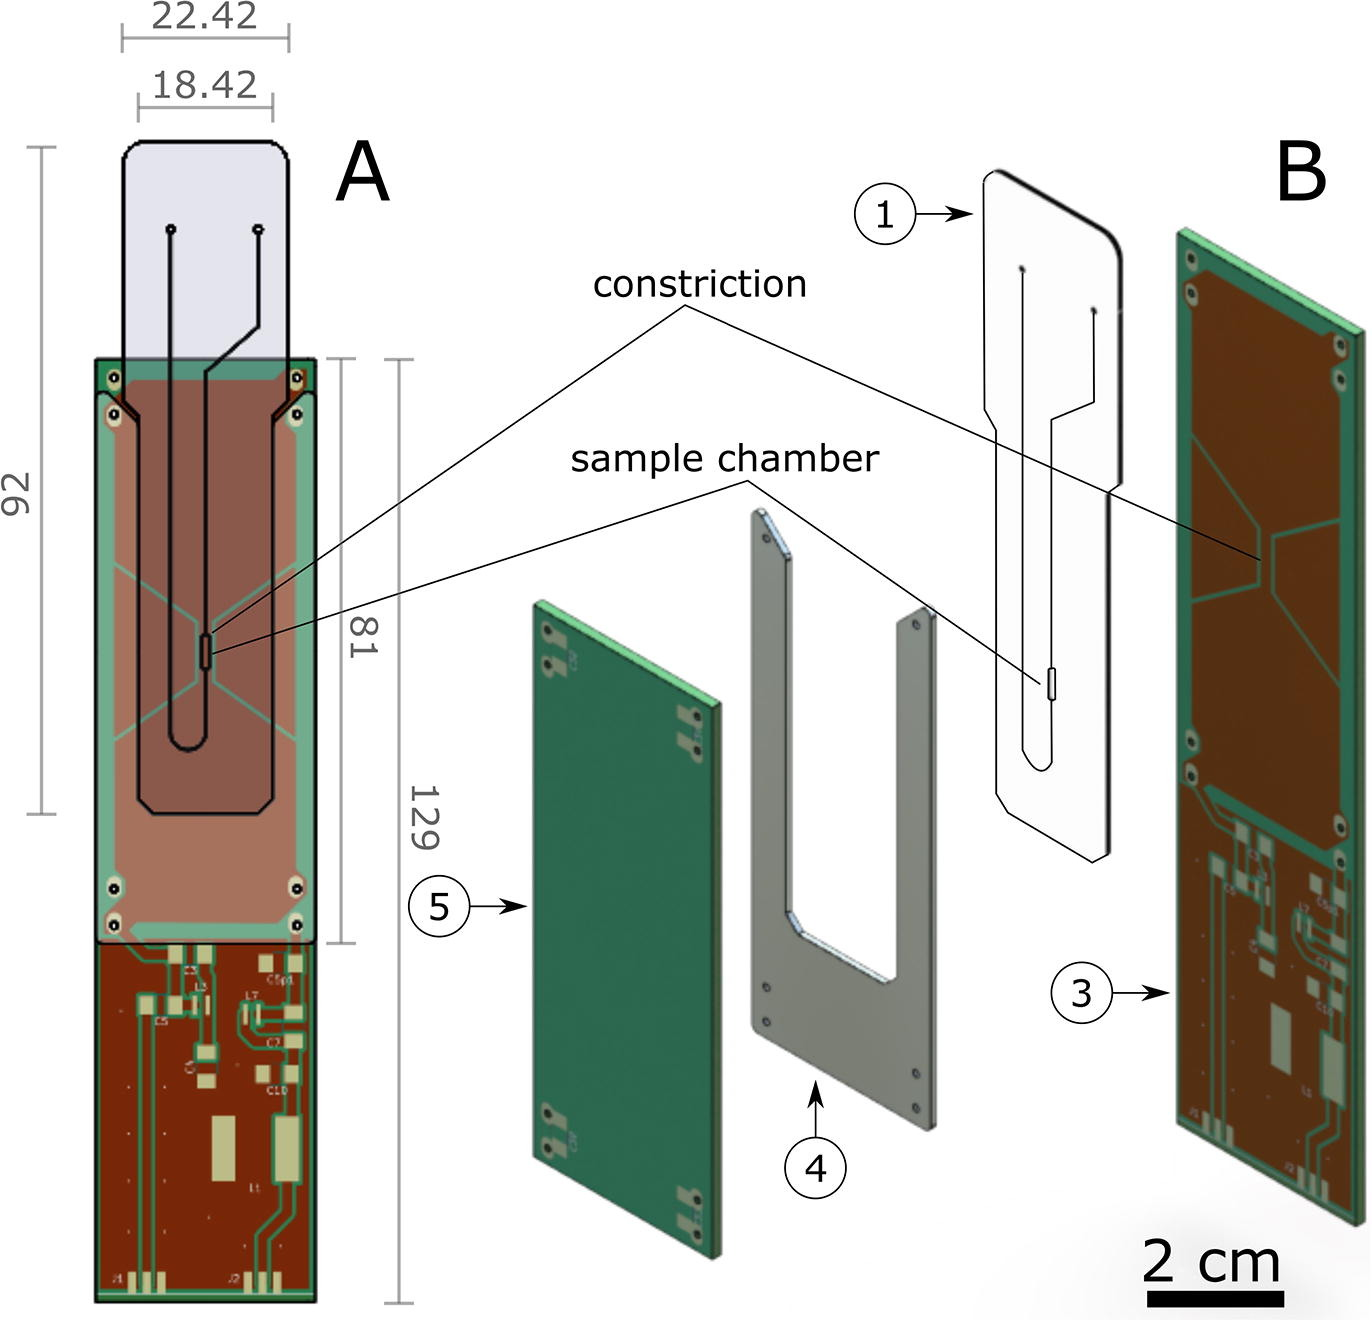
\includegraphics[width=\columnwidth]{Manvendra-Probe.jpg}
  \end{center}
  \caption{Drawings of the detector assembly and the microfluidic device (1). A: front view (dimensions in mm); B:
  exploded view. Spacer (4) ensures the alignment of the sample chamber with the constrictions on the PCB planes. In A,
  PCB plane 5 is hidden to show the orientation of 1 with respect to PCB plane 3. Thickness of each of the PCB planes
  is 1.52 mm and the copper layers on the PCBs is 35 $\mu~\text{m}$. Both the microfluidic device and the spacer are made from
  PMMA and have thickness of 0.9 mm and 1 mm respectively. Figure reproduced from\citep{RN164}}
  \label{fig:MVProbe}
\end{figure}
The main advantage of using this probe is the compatibility of the device with customisable chips allowing
a broad range of applications and enabling the marrying of practical NMR and some microfluidic capabilities which
few others allow\citep{RN165,RN166,RN167}. The limit of detection LOD for the TLP used is
1.4 nmol $\text{s}^{1/2}$ which comparitavely lower than detectors of a similar size and more similar to the LOD of
commercial cryo-probes mentioned previously. Where the probe is exceptional in terms of micro-detector is
the cLOD. Demonstrated in \fig{fig:cLOD}.
\begin{figure}
  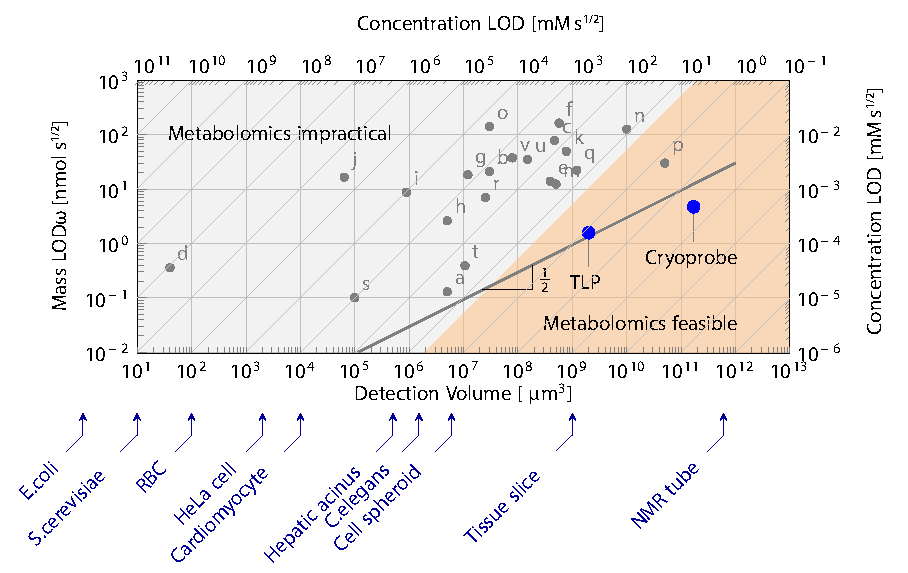
\includegraphics[width=\columnwidth]{sensitivity-ov.pdf}
  \caption{Plot comparing the limits of detection of previously design micro-NMR detectors. Letters
  a-t correspond to different authors as cited by Badilita \textit{et al.}\citep{Badilita:2011td} Letters u\citep{Meier:2014ds}
  and t\citep{RN165} represent more recent work. The probe used here is labelled at TLP and a comercial cyroprobe is shown for reference.}
  \label{fig:cLOD}
\end{figure}

For this work, the goal is not only to combine NMR detection and microfluidics, clearly that has been done before. However,
it is the combination of these two in a way that does not comprimise in either. That, in an NMR sense, means nLODs
comparible to macroprobes as well as sub 0.01 ppm line widths for true spectral resoltuion. This is displayed in
\fig{fig:cLOD}, the area shaded orange that we define as the 'metabolomics feasible' range is a maximum 5 mM $\sqrt{\text{s}}$
ensuring species present at 0.1 mM can be detected within less than 20 mins to a sufficient resolution. The TLP has a cLOD of
~ 1 mM $\sqrt{\text{s}}$ and can detect species at 0.02 mM in that time frame Whilst this is suitable for some metabolomic information to be
gained, however, the subtle changes in molecules present at less than 0.02 mM still evades us in the given time frame. Efforts towards
lowering the nLOD and cLOD are described in \ref{Parahydrogen}
